\documentclass[tikz,border=5pt]{standalone}
\usepackage[utf8]{vietnam}
\usepackage{amsmath,amssymb}
\usepackage{tikz}

\begin{document}
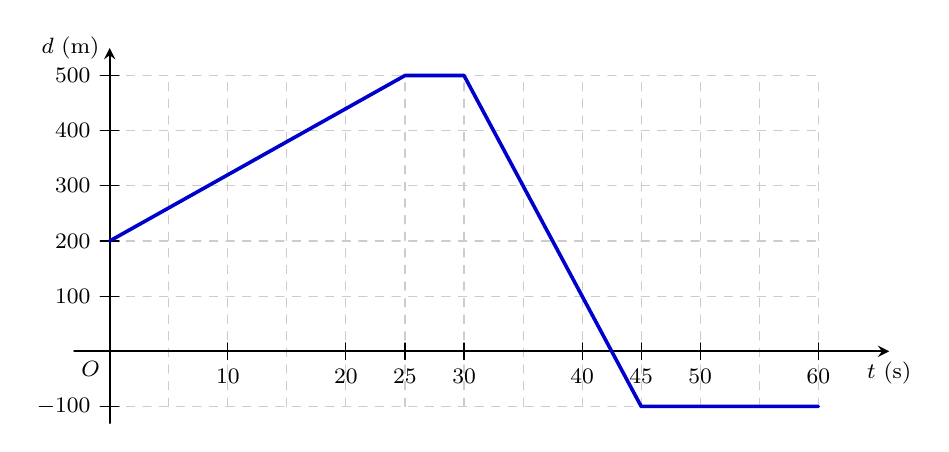
\begin{tikzpicture}[>=stealth, line join=round, line cap=round, font=\footnotesize, xscale=0.15, yscale=0.007]
	% Lưới tọa độ
	\draw[dashed, gray!40, thin] (0, -100) grid[xstep=5, ystep=100] (60, 500);

	% Hệ trục tọa độ
	\draw[->, thick] (-3, 0) -- (66, 0) node[below] {$t\text{ (s)}$};
	\draw[->, thick] (0, -130) -- (0, 550) node[left] {$d\text{ (m)}$};
	\node[below left] at (0, 0) {$O$};

	% Vạch chia trục hoành
	\foreach \t in {10, 20, 25, 30, 40, 45, 50, 60} {
		\draw (\t, 15) -- (\t, -15);
		\node[below] at (\t, -15) {$\t$};
	}

	% Vạch chia trục tung
	\foreach \d in {-100, 100, 200, 300, 400, 500} {
		\draw (0.8, \d) -- (-0.8, \d);
		\node[left] at (-0.8, \d) {$\d$};
	}

	% Đường đồ thị (d - t)
	\draw[line width=1.3pt, blue!80!black] (0, 200) -- (25, 500) -- (30, 500) -- (45, -100) -- (60, -100);

	% Đánh dấu các điểm mốc
	\foreach \p in {(0, 200), (25, 500), (30, 500), (45, -100), (60, -100)} {
		\fill[black] \p circle (2pt);
	}
\end{tikzpicture}
\end{document}
